\documentclass[paper=a0,accentcolor=tud9b,colorbacktitle,colorbacksubtitle]{tudposter} 
\usepackage{pdf14} 
%\usepackage[a-1b]{pdfx}
\usepackage{multicol} 
\usepackage{amsmath} 
\usepackage{graphicx} 
\usepackage{url} 
\usepackage{fancyhdr}
\usepackage{floatflt}
\usepackage{caption}
\usepackage{fancyhdr}

\pagestyle{fancy} 
\renewcommand{\titlesize}{\fontsize{97.0}{108.3}\selectfont} 
\addtokomafont{section}{\fontsize{42}{52}\selectfont} \SetMathAlphabet{\mathcal}{normal}{OMS}{cmsy}{m}{n}

% Title Page
\title{\color{white} Fast System Identification for Barrier Bucket Input Signal Generation*} \subsubtitle{\color{white}J. Harzheim, D. Bast, D. Domont-Yankulova, M. Frey, A. Galetzka, K. Gro{\ss}, H. Klingbeil}

\begin{document} 
\fontsize{28}{32}\selectfont 
\maketitle \setlength{\columnsep}{3em} ~\\[-2.5em]
\begin{multicols}{2}
	

\section{Introduction}
	 %At GSI, Barrier Bucket RF systems are currently designed for the SIS 100 synchrotron (part of the future accelerator 
	 %facility FAIR) and the Experimental Storage Ring (ESR). In order to facilitate a large variety
	 
	 \vspace{0.3cm}
	 \hspace{-0.6cm}
	 \begin{minipage}{0.17\textwidth}	  
	 At GSI, Barrier Bucket RF systems are currently designed for the SIS 100 synchrotron (part of the future accelerator 
	 facility FAIR) and the Experimental Storage Ring (ESR). In order to facilitate a large variety of longitudinal bunch 
	 manipulations these systems have to provide 
	 high quality single-sine gap voltages (right-handed figure).
	 To achieve the desired output signal quality, a proper mathematical modeling of the system is needed to estimate the required input signal.
	 %To estimate the required input signal for the desired output signal quality, a proper mathematical modeling of the system is needed. 
	 \end{minipage}
	 %\begin{minipage}{0.01}
	 %\vspace{0.1cm} 
	 %\end{minipage}
	 \begin{minipage}{0.34\textwidth}
	 \hspace{0.4cm}
	 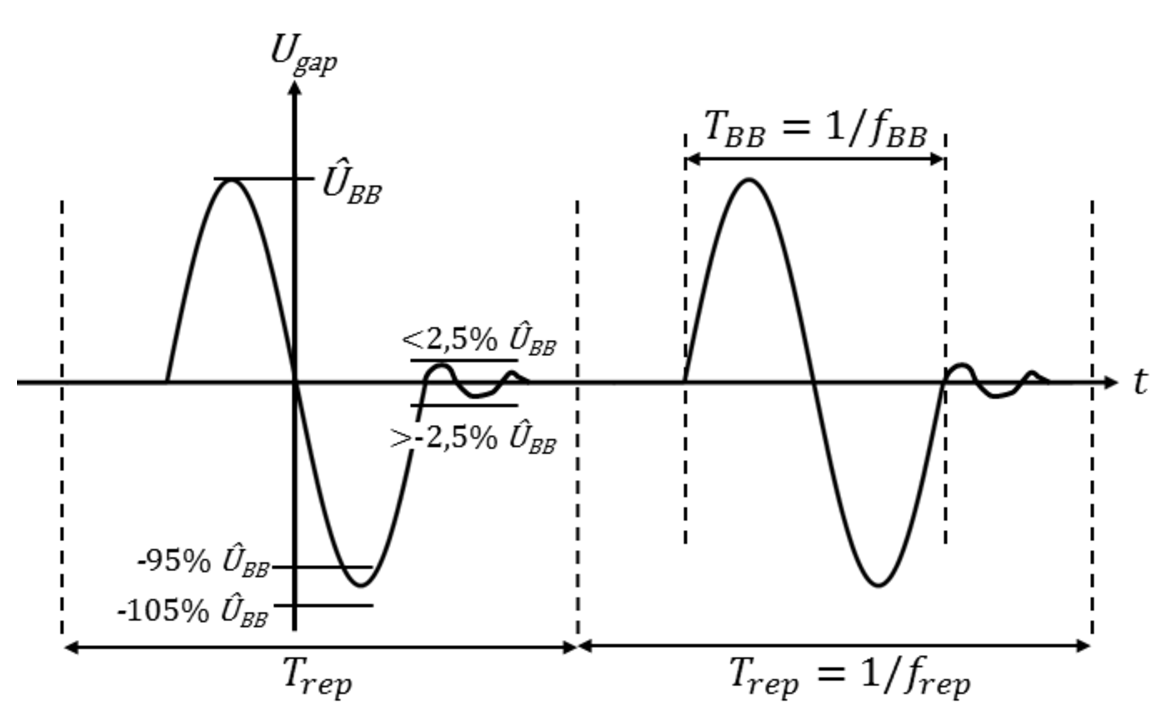
\includegraphics[scale=1.2]{WEPVA047f1.eps}
	 \captionof*{figure}{Desired output gap voltage.}
	 \label{bb_signal}
	 \end{minipage}
	 	
	\section{Linear region}	
	%\begin{itemize}
	 Fourier decomposition of the ideal output signal yields
	 \fontsize{33}{40}
	      \begin{equation*}
	      \textstyle
		U_{out}(t)=\sum \limits_{n=1}^\infty \underbrace{\hat{U}\frac{T_{BB}}{T_{rep}}\left[\text{si}\left(\pi\left[n\frac{T_{BB}}{T_{rep}}+1\right]\right)-
		\text{si}\left(\pi\left[n\frac{T_{BB}}{T_{rep}}-1\right]\right)\right]}_{b_{n,\text{out}}}\cdot \text{sin}(n\omega_{rep}t).
	      \label{U_out}
	      \end{equation*}
	 \fontsize{35}{40}     
	 In the linear region $\textstyle \underline{U}_{in}(\omega)=\underline{U}_?(\omega)=\underline{U}_{out}(\omega)/\underline{H}(\omega)$ holds. The frequency
	 response $\textstyle \underline{H}(\omega)$ is measured using Pseudo Random Binary Signals (PRBS) as input. Such signals can be generated using a shift register, 
	 which is shown for a register of the length $\textstyle b=7$ hereafter.
	 
	 \begin{center}	
	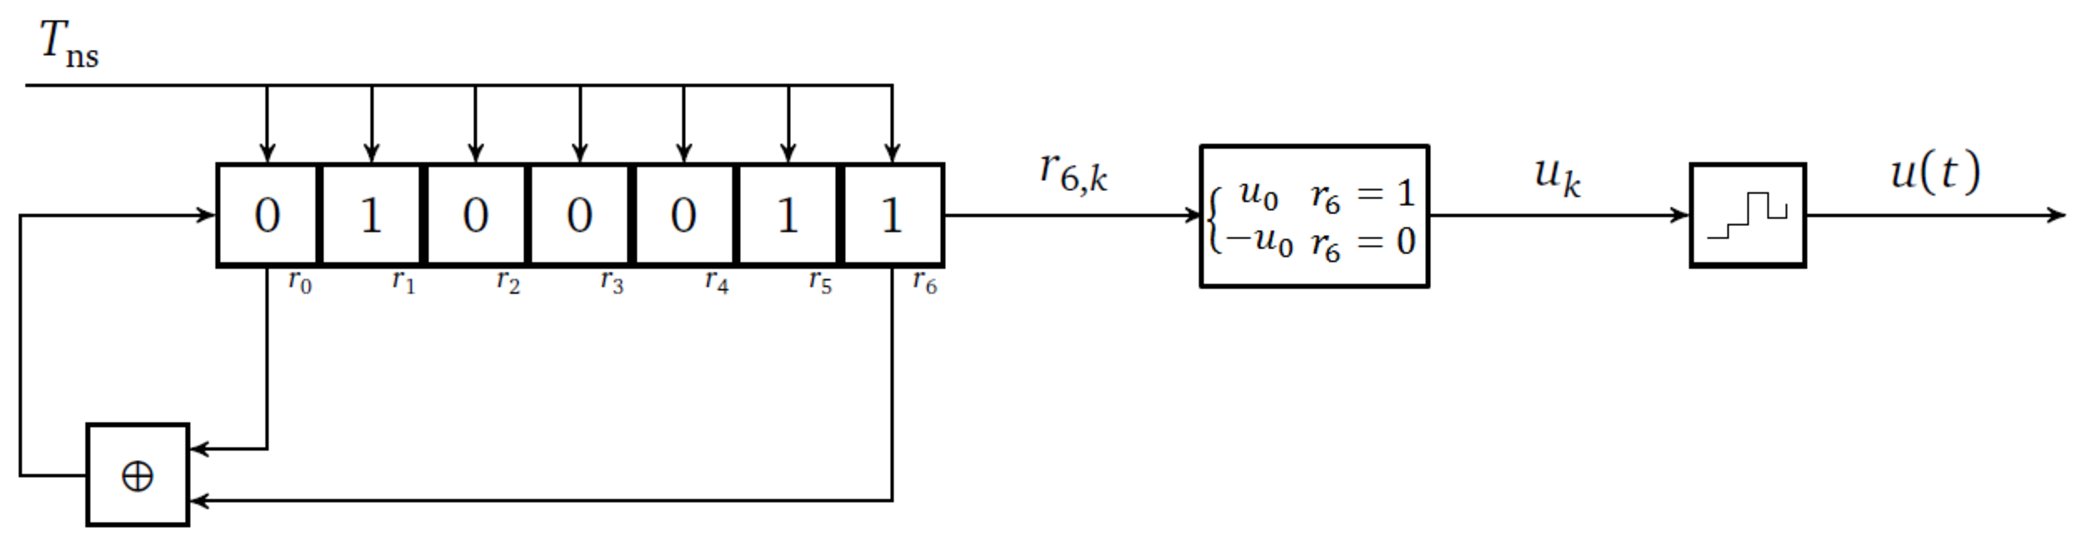
\includegraphics[scale=1.1]{Schieberegister.eps}
	\captionof*{figure}{Shift register of length $b=7$}
	\label{Modellierung}
%    	\vspace*{-\baselineskip}
	\end{center}
	 
	 %\end{itemize}
	 \begin{minipage}{0.195\textwidth}
	 Two parameters can be varied to change the signal properties: The length $\textstyle  b$ and the clock frequency $\textstyle f_{ns}$ of the register.
	 $\textstyle f_{ns}$ is given by the maximum frequency, which has to be measured. As the PBRS  spectrum can  be described by
	 	 \vspace{-0.5cm}
	 \begin{equation*}
	 \textstyle
	  |\underline{u_l}|=
	  %\begin{cases}
	  % \frac{U_0}{N_n} \qquad \textrm{f\"ur l=0} \\
	   U_0 \sqrt{\frac{N_n+1}{N_n}}\left| \textrm{si}\left(\frac{l\cdot T_{ns}\cdot \pi}{T_P} \right) \right|,
	  %\end{cases}
	 \end{equation*}
	\end{minipage}
	\begin{minipage}{0.01\textwidth}
	 \hspace{1cm}
	\end{minipage}
	\begin{minipage}{0.34\textwidth}
	 \begin{center}
	 \hspace{-4.5cm}
	  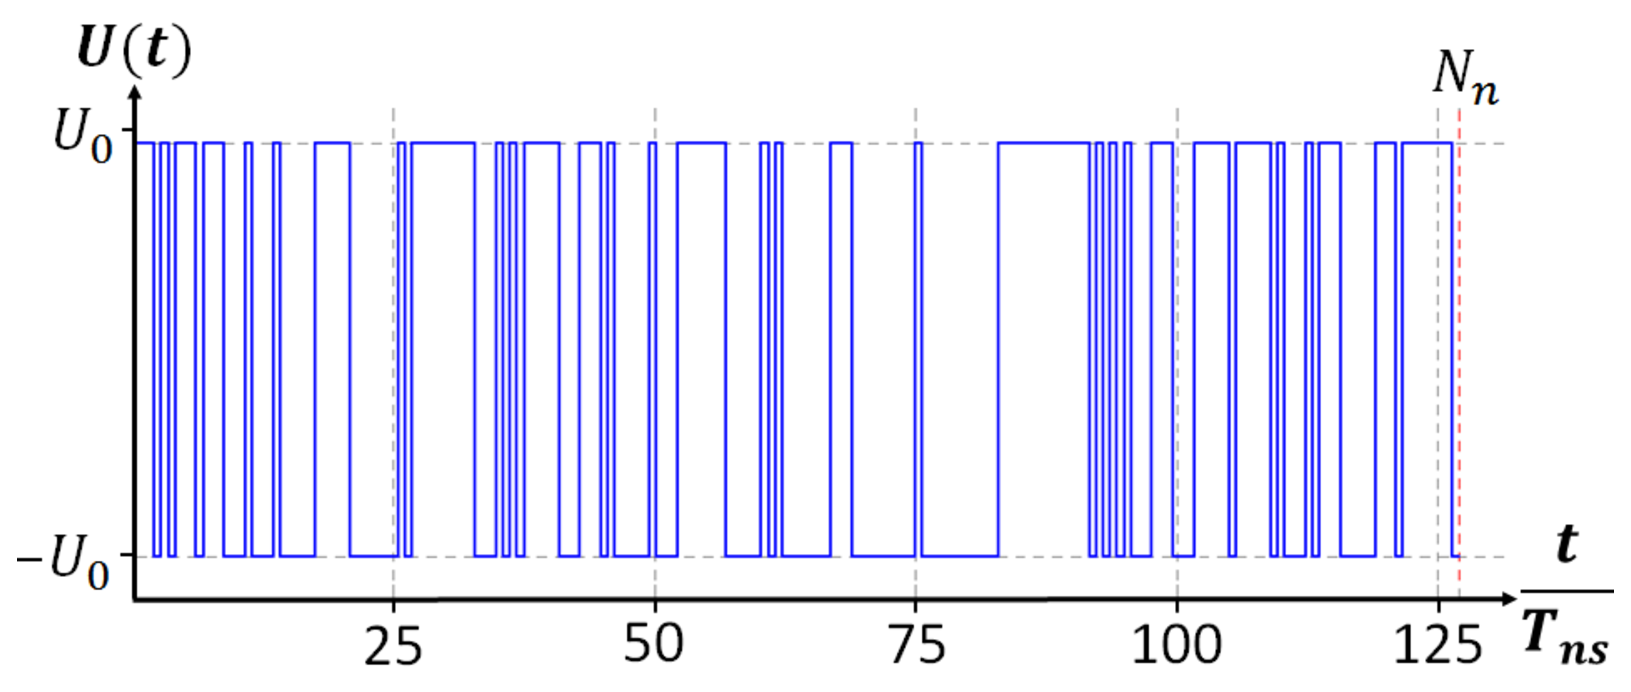
\includegraphics[scale=0.75]{PBRS_Signal3.eps}
	  %\vspace{-1cm}
	  \captionof*{figure}{PRBS input signal ($b=7$)} 
	  \label{H_ESR}
	  %\vspace*{-0.5cm}
	 \end{center}
	 \end{minipage}
	 
	 %\end{itemize}
	 \begin{minipage}{0.195\textwidth}
	 %\vspace{-1.2cm}
	$\textstyle f_{ns}=2,5\cdot f_{max}=2,5\cdot 80\textrm{ MHz}$ is chosen. $\textstyle b$ determines the signal length $\textstyle T_P=N_n\cdot T_{ns}$ 
	with ${\textstyle N_n=2^b-1}$  
	and therefore defines the frequency resolution $\textstyle f_p$ of the measurement. Thus,
	\vspace{-0.5cm}
	\begin{equation*} 
	\textstyle
	 b=\left\lceil \ln \left( 2,5 \frac{f_{max}}{f_{p,min}}+1 \right)  \ln(2) \right\rceil
	 	\vspace{-1cm}
	\end{equation*}
	can be used to estimate $\textstyle b$.
	\end{minipage}
	\begin{minipage}{0.01\textwidth}
	 \hspace{1cm}
	\end{minipage}
	\begin{minipage}{0.34\textwidth}
	 %\vspace{-0.5\baselineskip}
	\begin{center}
	\hspace{-5cm}
	 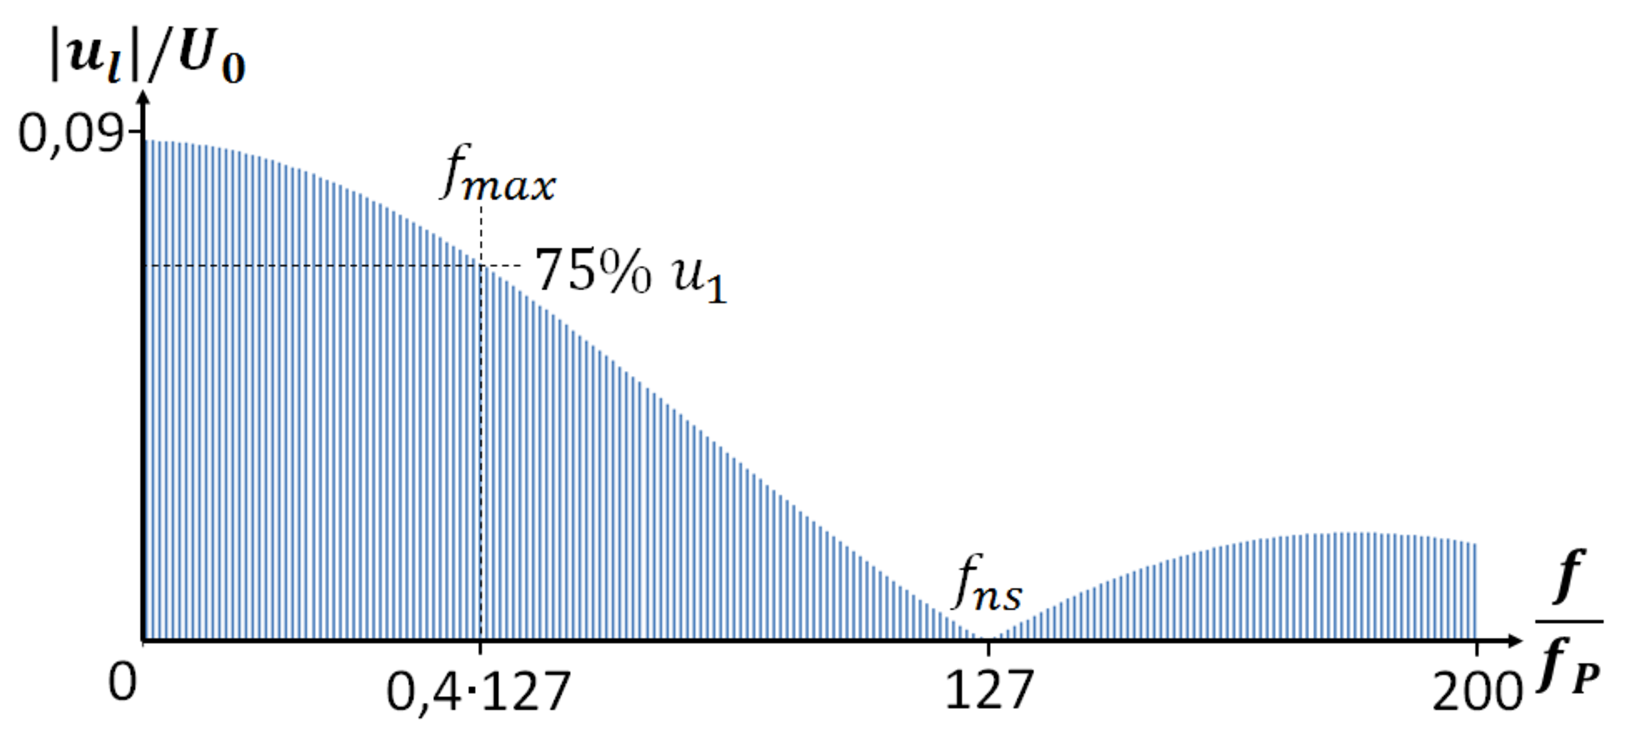
\includegraphics[scale=0.8]{PBRS_Spektrum3.eps}
	  \label{Signal}

	  \captionof*{figure}{PRBS spectrum ($b=7$)}	  	 
	\end{center}
	%\vspace{\baselineskip}
	 \end{minipage}
	 
	 %\end{itemize}
	 \begin{minipage}{0.24\textwidth}
	 \begin{center}
	  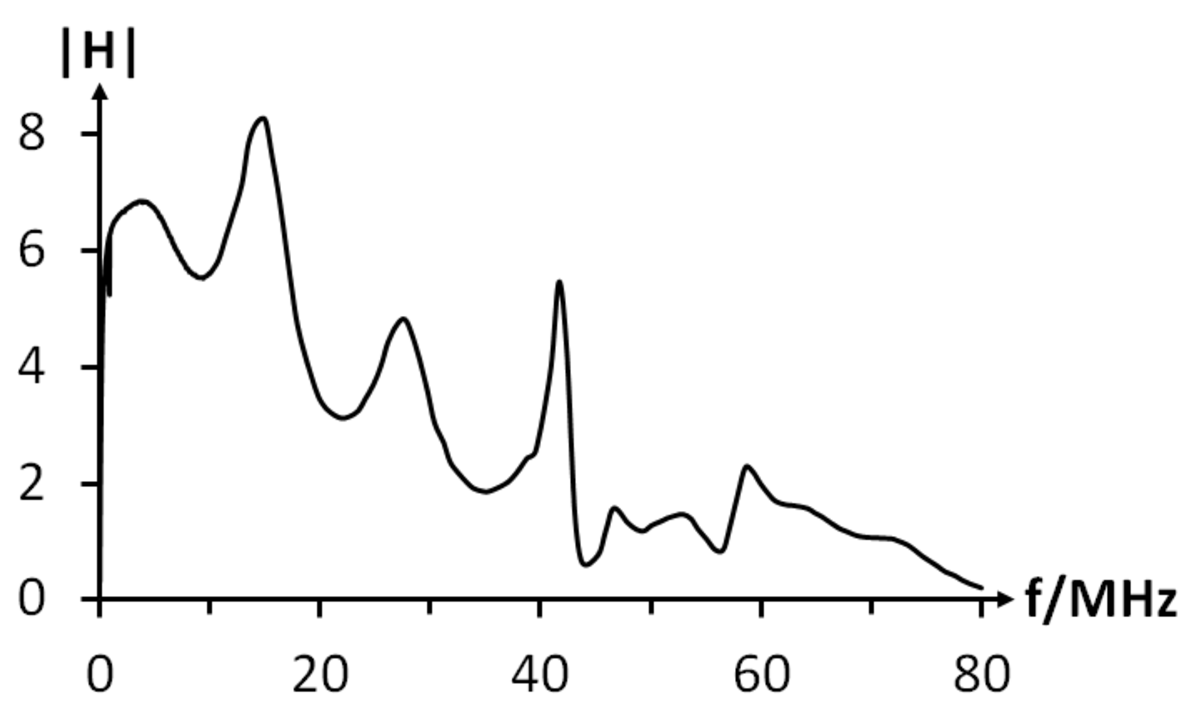
\includegraphics[scale=0.9]{WEPVA047f3_2.eps}
	  %\vspace{-1cm}
	  \captionof*{figure}{Measured amplitude response of the ESR BB prototype system.} 
	  \label{H_ESR}
	  %\vspace*{-0.5cm}
	 \end{center}
	\end{minipage}
	\begin{minipage}{0.01\textwidth}
	 \hspace{1cm}
	\end{minipage}
	\begin{minipage}{0.22\textwidth}
	 %\vspace{-0.5\baselineskip}
	\begin{center}
	 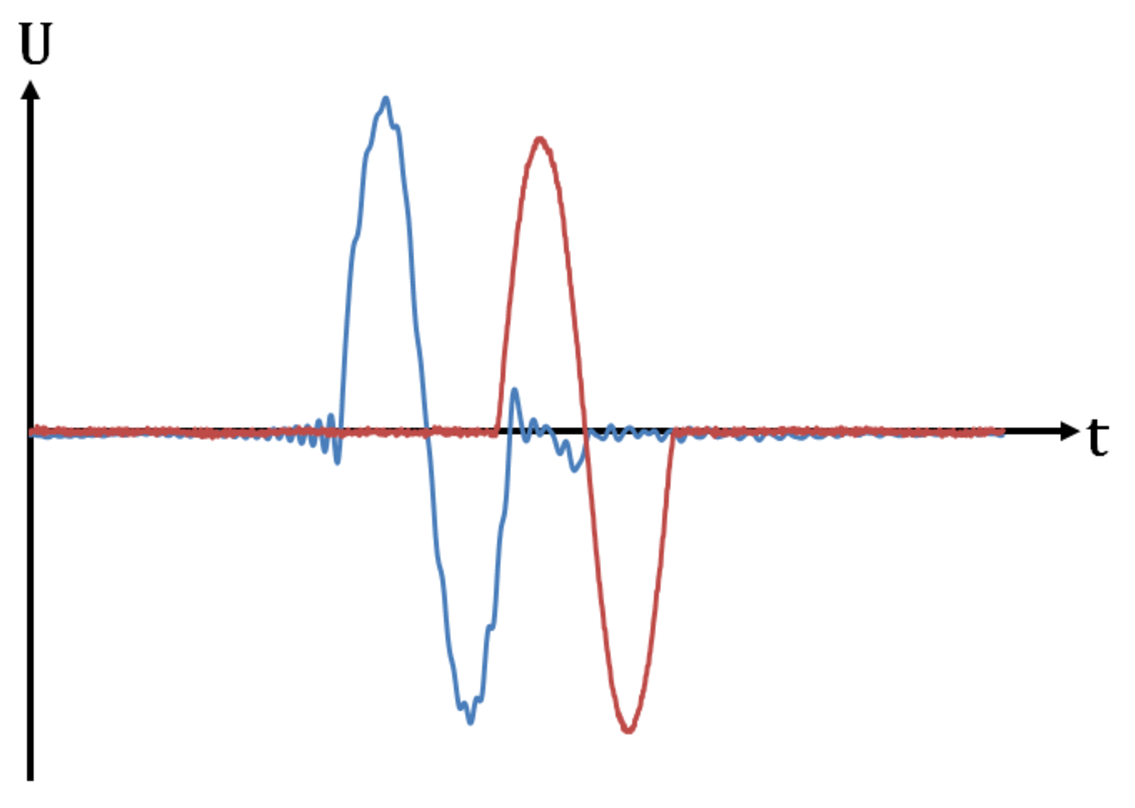
\includegraphics[scale=0.8]{U_BB_KWT2017_2.eps}
	  \label{Signal}
	  %\vspace{-1.5cm}
	  \captionof*{figure}{Measured input and output signal in the linear region ($\hat{U}_{BB}=520\,V$).}	  	 
	\end{center}
	%\vspace{\baselineskip}
	 \end{minipage}
	 
	 


	
	\section{Nonlinear Approach}	
	\begin{center}	 
	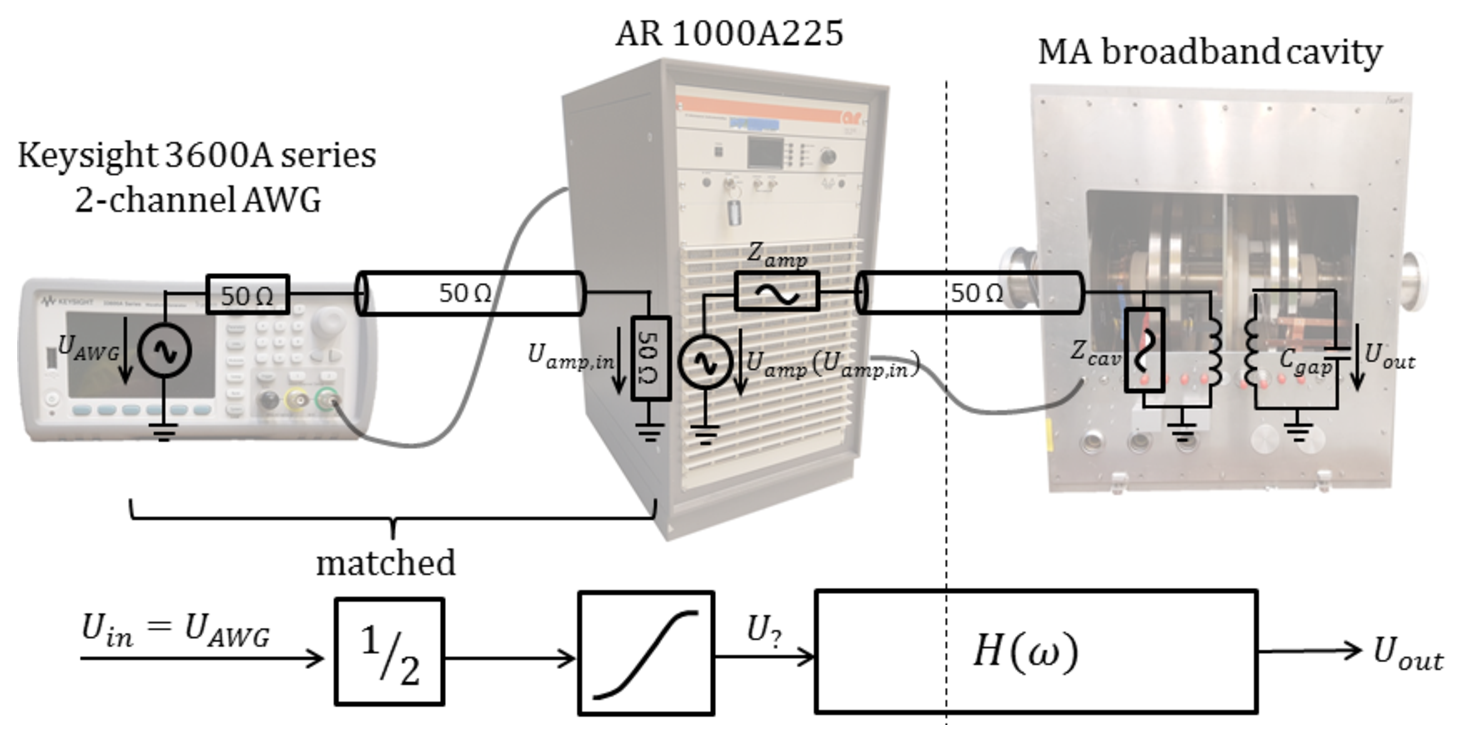
\includegraphics[scale=1.2]{WEPVA047f2_2.eps}
	\captionof*{figure}{Hammerstein modeling of the ESR BB prototype system.}
	\label{Modellierung}
%    	\vspace*{-\baselineskip}
	\end{center}
	%\begin{itemize}
	 To characterize the static nonlinearity, a power series ansatz was chosen:
	 \vspace{-0.4cm}
	    \begin{equation*}
	    \textstyle
	      U_?(t)=f\left(U_{in}(t)\right)=\sum_{n=1}^N a_n \left[ U_{in}(t) \right]^n.
	      \label{Potenzreihe}
	    \end{equation*}
	 As $\textstyle U_?(t)$ can't be measured directly, it is calculated from $\textstyle U_{out}(t)$ using
	 $\textstyle\underline{U}_?(\omega)=\underline{U}_{out}(\omega)/\underline{H}(\omega)$. Afterwards, the coefficients $a_n$ can be calculated
	 by solving the linear optimization problem
		\begin{equation*}
		\textstyle
	  \left( 
	 \begin{matrix}
	  U_{in,1} & U_{in,1}^2 & \dots & U_{in,1}^N \\
	  U_{in,2} & U_{in,2}^2 & \dots & U_{in,2}^N \\
	  \vdots & \vdots & \ddots & \vdots \\
	  U_{in,M} & U_{in,M}^2 & \dots & U_{in,M}^N \\
	 \end{matrix}
	\right)
	\cdot
	\left(
	\begin{matrix}
	 a_1 \\
	 a_2 \\
	 \vdots \\
	 a_N \\	 
	\end{matrix}
	\right) 
	= \left( 
	\begin{matrix}
	 U_{?,1} \\
	 U_{?,2} \\
	 \vdots \\
	 U_{?,M} \\	 
	\end{matrix}
	\right).
	\label{lgs}
	\end{equation*}
	
	\hspace{-0.7cm}
	\begin{minipage}{0.17\textwidth}
	 with $\textstyle U_{in}(t)$ and $U_?(t)$ consisting of $\textstyle M$ samples. Best output signals were achieved using 3rd or 4th order power series and
	 a linearly presdistorted testsignal.
	 The inverse characteristic $\textstyle f^{-1}$ can be calculated from measurement data and is stored in form of a look-up table.\\
	 With the measured frequency response $\textstyle \underline{H}(\omega)$ and the inverse characteristic $\textstyle f^{-1}$,  the input signal is computed as shown
	below.
	\end{minipage}
	\begin{minipage}{0.33\textwidth}
	\vspace{-0.5cm}
	 \begin{center}
	  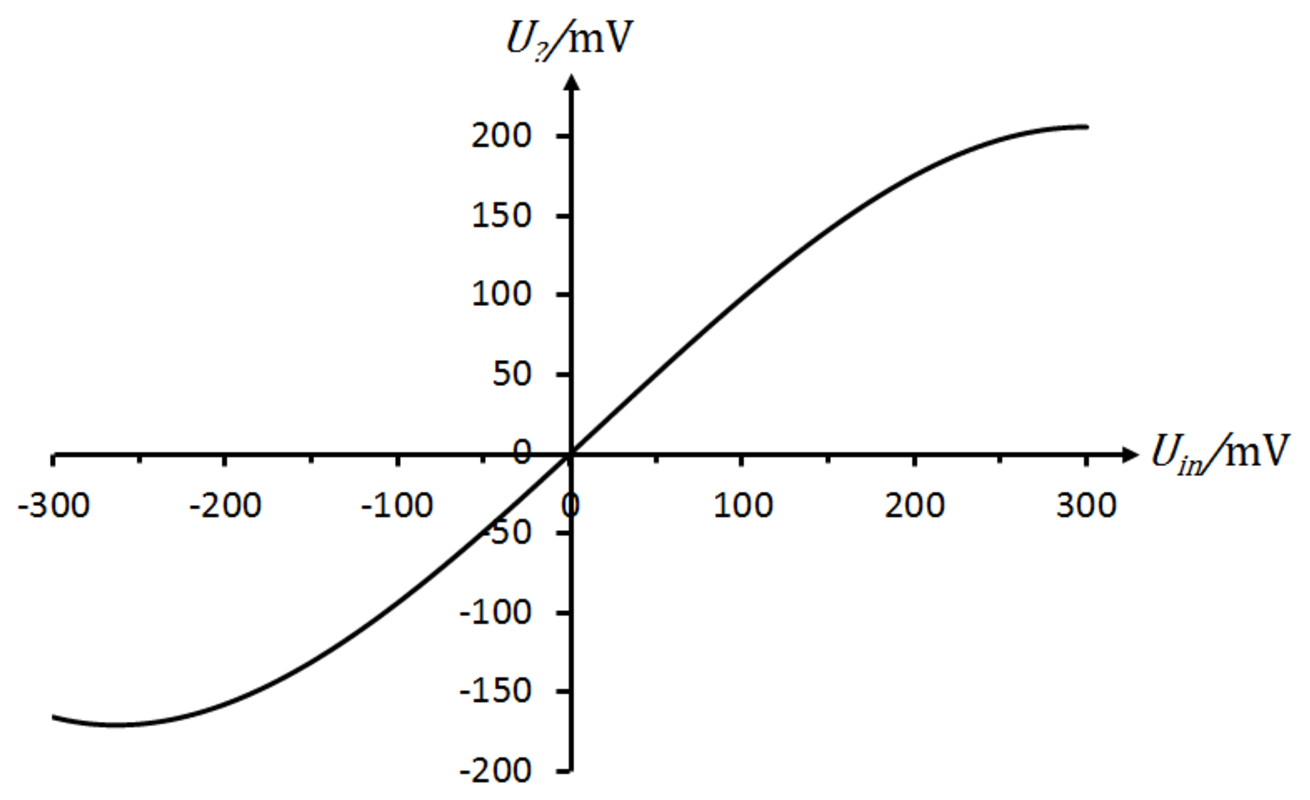
\includegraphics[scale=1]{WEPVA047f6.eps}
	 \label{Kennlinie}
	 %\vspace{-1cm}
	 \captionof*{figure}{Measured 3rd order polynomial nonlinearity.}
	 \end{center}
	 \vspace{0.1cm}
	\end{minipage}
	
	\vspace{0.5cm}
	\begin{center}
	 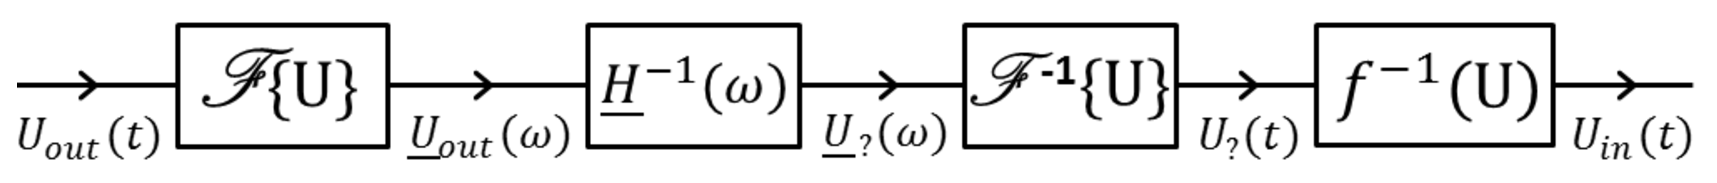
\includegraphics[scale=1.3]{WEPVA047f3_8.eps}
	 \label{Signalchain}
	 \vspace{-0.3cm}
	 \captionof*{figure}{Different steps to compute the input signal $U_{in}(t)$ for a desired output $U_{out}(t)$}
	\end{center}
	 	
	\section{Results}
       %\vspace*{1cm}
	\begin{center}
	%\vspace{-1cm}
	 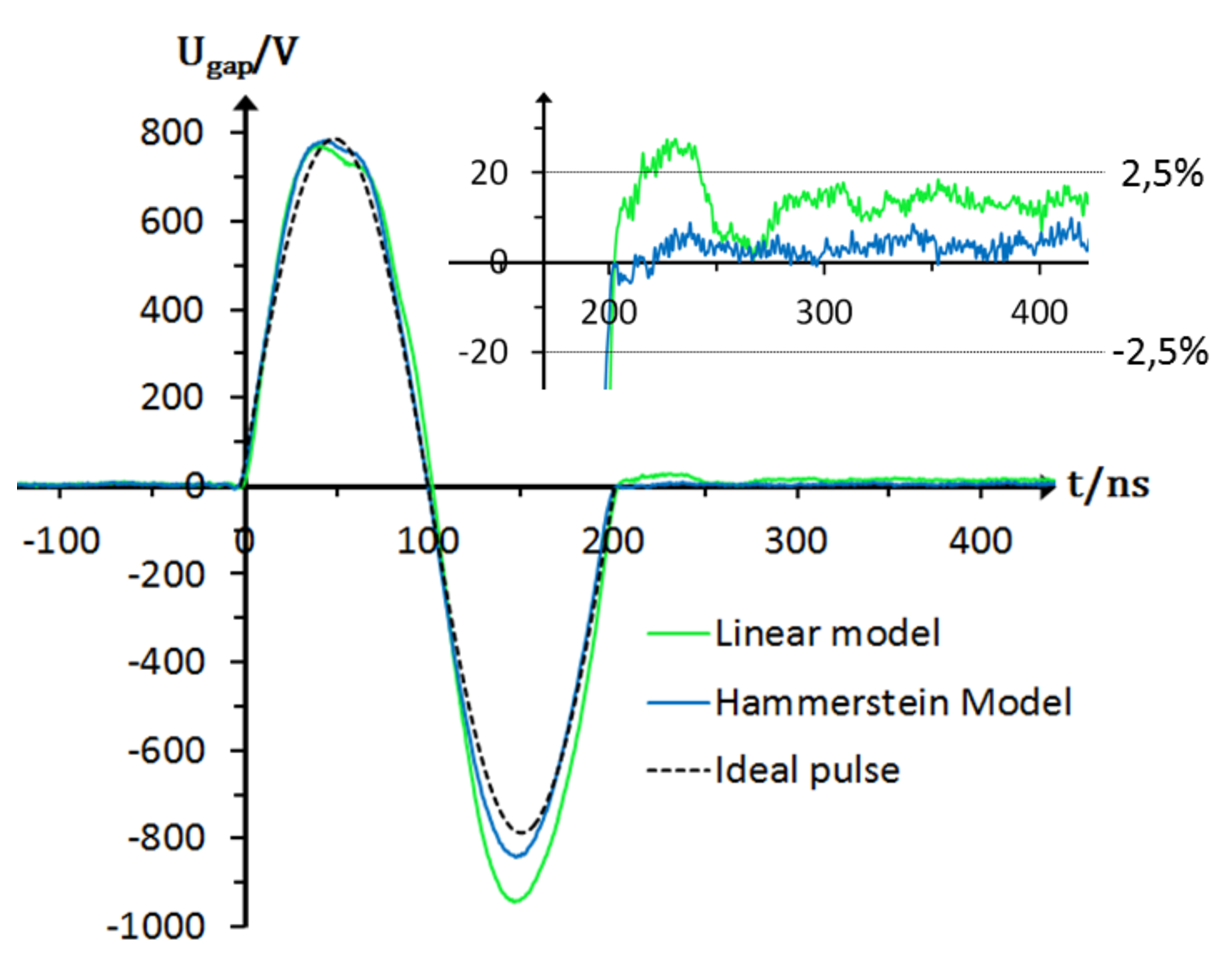
\includegraphics[scale=1.2]{WEPVA047f7.eps}
	 \label{Vergleich}
	 %\vspace{-0.2cm}
	 \captionof*{figure}{Resulting voltages for linear and nonlinear predistortion for $\hat{U}=800\,V$.}
	 \end{center}	 
	 %\vspace*{1cm}
	%\end{figure} 
	\begin{minipage}{0.24\textwidth}
	 \begin{itemize}
	 \item Reduction of ringing to below 1\%.
	 \item Reduction of difference in half-cycles from 22\% to 7\%.
	 \end{itemize}
	\end{minipage}
	\begin{minipage}{0.25\textwidth}
	 \begin{itemize}
	 \item Fulfills requirements for $\textstyle \hat{U}_{out}(t)<760$ V.
	 \item Reduction of measurement time from >1\,h to <1\,min.
	 \end{itemize}
	\end{minipage}



%----------------------------------------------------------------
%\newpage

\iffalse  % only for "biblatex"
	\newpage
	\printbibliography

% "biblatex" is not used, go the "manual" way
\else

%\begin{thebibliography}{99} % Use for 1-9 references

%\bibitem{accelconf-ref}
%	C. Petit-Jean-Genaz and J. Poole,
%	``JACoW, A service to the Accelerator Community,''
%	EPAC'04, Lucerne, July 2004, THZCH03,  p.~249,
%	\url{http://www.JACoW.org/e04/papers/THZCH03.PDF}
%\bibitem{FAIR}
%	H. H. Gutbrod \textit{et al.}, “FAIR - Baseline Technical Report, Volume 2, Accelerator and Scientific Infrastructure“,
%	GSI, Darmstadt, Germany, September 2006.
			
%\bibitem{Demo_BB_ESR}
%	M. Steck \textit{et al.}, “Demonstration of Longitudinal Stacking in the ESR with Barrier Buckets and Stochastic Cooling“,
%	in \textit{Proc. COOL 2011}, Alushta, Ukraine, September 2011, paper TUPS20, pp. 140-143.
	
%\bibitem{BB_Fermilab}
%	C. M. Bhat, “Applications of barrier bucket RF systems at Fermilab“,
%	FNAL, Batavia IL, USA, Rep. FERMILAB-CONF-06-102-AD, March 2006.
	
		
%\bibitem{BB_dynamics}
%	C. M. Bhat, “Particle dynamics in storage rings with barrier rf systems“,
%	in \textit{Physical Review}, Vol.~55, Iss.~5, May 1997.
	
%\bibitem{Buch_HK}
%	H. Klingbeil, U. Laier and D. Lens, “Theoretical Foundations of Synchrotron and Storage Ring RF Systems“,
%	Springer, Heidelberg, Germany, 2015.
	
%\bibitem{BB_dynamics_synchrotron}
%	C. M. Bhat, “Barrier rf systems in synchrotrons“,
%	FNAL, Batavia IL, USA, Rep. FERMILAB-CONF-04-091-AD, 2004.
		
%\bibitem{MOV_B2}
%	O. Boine-Frankenheim, “RF barrier compression with space charge“,
%	in \textit{Physical Review} ST Accel. Beams 13, 034202,
%	Germany, March 2010.
	
%\bibitem{Mov_B1}	
%	M. Krestnikov \textit{et al.}, “Particle Accumulation Using Barrier Bucket RF System“,
%	in \textit{Proc. COOL'09}, Lanzhou, China, 2009, paper TUM2MCIO02, pp. 67-70.
	
%\bibitem{Paper_Frey}
%	M. Frey, D. Domont-Yankulova, J. Harzheim, K. Groß and H. Klingbeil, “Prototype Results of the ESR Barrier Bucket System“,
%	in \textit{Proc. IPAC'17}, Copenhagen, Denmark, May 2017, paper THPIK015, this conference.
	
%\bibitem{Paper_Gross}
%	K. Gross, D. Domont-Yankulova, M. Frey, J. Harzheim and H. Klingbeil, “Test Setup for Automated Barrier Bucket Signal Generation“,
%	in \textit{Proc. IPAC'17}, Copenhagen, Denmark, May 2017, paper THPAB098, this conference.

	
%\bibitem{ring_core}
%	S. Jatta, “Umgebungseinfluss bei Messungen  mit MA-Ringkernen“,
%	GSI internal report,
%	GSI Darmstadt, Germany, 2013.
	
%\bibitem{vector_fitting}
%	B. Gustavsen a	B. Gustavsen and A. Semlyen, “A robust approach for system identification in the frequency domai“
%	in \textit{IEEE Trans. Power Delivery}, vol. 19, no. 3, pp. 1167-1173, July 2004.	
	
%\bibitem{vec_f1}
%	B. Gustavsen and A. Semlyen, “Enforcing passivity for admittance matrices approximated by rational functions“,
%	in \textit{IEEE Trans. Power Systems}, vol. 16, no. 1, pp. 97-104, February 2001.
	
%\bibitem{vec_f2}
%	B. Gustavsen, “Computer code for rational approximation of frequency dependent admittance matrices“, 
%	in \textit{IEEE Trans. Power Delivery}, vol. 17, no. 4, pp. 1093-1098, October 2002.
	
%\bibitem{RK_2}
%	C. Ohmori \textit{et al.}, “A wideband RF cavity for JHF synchrotrons“, 
%	in \textit{Proc. Particle Accelerator Conference 1997}, Vancouver, BC, Canada, May 1997, pp. 2995-2997.

%\bibitem{RK_1}
%	T. Trupp, “NANOPERM® Broad Band Magnetic Alloy Cores for Synchrotron RF Systems“,
%	in \textit{Proc. IPAC2014}, Dresden, Germany, 2004, paper MOPRO016, pp. 95-98.	
	
%\bibitem{Harzheim:IPAC2016-MOPMW002}
%	J. Harzheim, D. Domont-Yankulova, M. Frey, H. Klingbeil, and R. Königstein,
%	\textquotedblleft{Modeling and Simulation of Broadband RF Cavities in PSpice}\textquotedblright,
%	in \textit{Proc. IPAC’16},
%	Busan, South Corea, May 2016, 
%	paper MOPMW002, pp. 392--395.	
	
%\bibitem{SIS100_spec}
%	GSI PBRF Department, “Detailed Specification of the SIS100 Barrier Bucket System for FAIR“,
%	GSI internal report, GSI Darmstadt, Germany, August 2016.
   
%\bibitem{HESR_BB}
%	R. Stassen \textit{et al.}, “The HESR RF-system and tests in COSY“,
%	in \textit{Proc. EPAC08}, Genoa, Italy, 2008, paper MOPC125, pp. 361-363.
	
%\bibitem{gross}
%	S. Jatta and K. Gross, “Spectrum of the BB signal at different periodicities“,
%	GSI internal report, GSI Darmstadt, Germany, November 2013. %\newline	
	
%\bibitem{VV_JH}
%	J.~Harzheim, “Zusammenfassung nichtlineare Vorverzerrung“,
%	GSI internal report, GSI Darmstadt, Germany, December 2016.
	
%\bibitem{Buch_Nonl}
%	O.~Nelles, “Nonlinear System Identification“,
%	Springer, Heidelberg, Germany, 2001.\\
	
%\bibitem{Ham1}
%	P. Gilabert, G. Montoro, and E. Bertran. "On the Wiener and Hammerstein models for power amplifier predistortion." 
%	in \textit{Proc. APMC’05}, Suzhou, China, December 2005.
	%Microwave Conference Proceedings, 2005. APMC 2005. Asia-Pacific Conference Proceedings. Vol. 2. IEEE, 2005.
	
%\bibitem{Ham2}
%	Isaksson, Magnus, David Wisell, and Daniel Ronnow. "A comparative analysis of behavioral models for RF power amplifiers." 
%	IEEE transactions on microwave theory and techniques 54.1, 2006, pp. 348-359.
	

	
%\end{thebibliography}
%\null  % this is a hack for correcting the wrong un-indent by package 'flushend' in versions before 2015

%\null 	
	  
\end{multicols}
\vspace{3cm}
\fancyfoot{}
\renewcommand{\footruleskip}{15pt} 
\begin{picture}
	(0,0) \put(-10,85){\rule{1.0\hsize}{2.2pt}} 
\end{picture}
\lfoot{\vspace{-3.5cm} \normalsize{ \textbf{Technische Universit\"at Darmstadt}\\
Institut f\"ur Theorie Elektromagnetischer Felder\\
Schlo{\ss}gartenstr. 8, 64289 Darmstadt\\
www.temf.tu-darmstadt.de}}
%\newline
%\normalsize{Work partly funded by}
\cfoot{ \vspace{-4cm} \normalsize{* Work partly funded by}% \newline}
%\newline \normalsize{Work partly funded by}
%}
%\newline
%\vspace{-8cm}
%\hspace{-8cm}
%\cfoot{
\begin{picture}(0,0)
  \put(-420,-140){
\includegraphics[scale=0.25]{BMBF-logo.eps}}
  \put(-90,-80){
\includegraphics[scale=0.12]{GSI-logo.eps}}
\end{picture}
}
\rfoot{\vspace{-3.5cm} 
\begin{picture}
	(0,0) \put(-150,-130){

\includegraphics[width=5.2cm]{temf-logo}}
\end{picture}
}


\end{document} 
